\documentclass{article}
\usepackage[utf8]{inputenc}
\usepackage{graphicx}
\title{Assignment 4 Project Management Agile Development}
\author{Team: Dynmo }
\begin{document}

\maketitle
\section{Team Members}
\subsection{Nisha Nisha-C0736218}  
\subsection{Gurjant Singh- C0740004}
\subsection{Amandeep Kaur-C0735316}
\subsection{Harkaran Singh- C0737550}

\centering
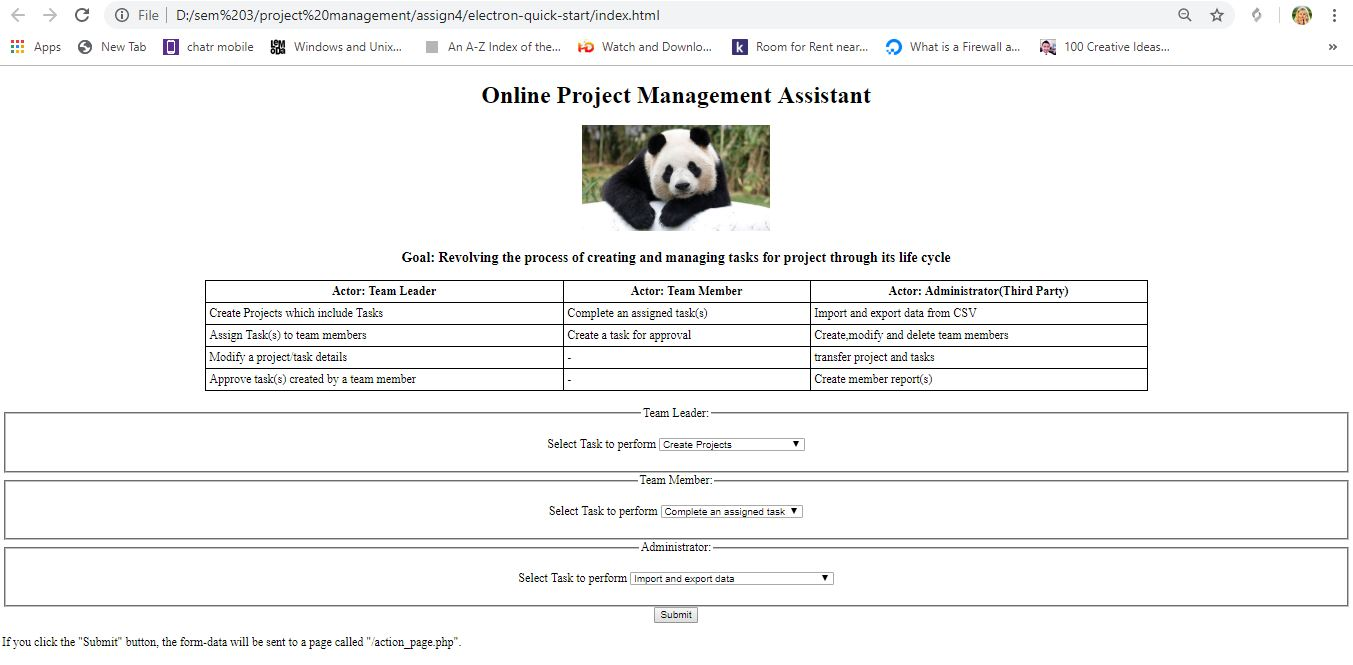
\includegraphics[width=9cm, height=9cm]{html page panda.JPG}
\section * {Our Web Application Code:}
\begin{verbatim}
   <!DOCTYPE html>
<html>
  <head>
      <style>
          table, th, td 
          {
            border: 1px solid black;
            border-collapse: collapse;          
          }
      </style>
    <meta charset="UTF-8">
    <title>Project Assignment</title>
  </head>
  <body>
    <h1><center>Online Project Management Assistant</center></h1>
    <center><img src="D:\sem 3\project management\assign4\electron-quick-start\panda.jpg"width="250">
    </center> 
    <h3><center>Goal: Revolving the process of creating and managing tasks for project through its life cycle</center></h3>
    <center><table style="width:70%" cellpadding="5"cellspacing="5">
    <center>
    <tr>
          <th>Actor: Team Leader</th>
          <th>Actor: Team Member</th> 
          <th>Actor: Administrator(Third Party)</th>
    </tr></center>
    <tr>
          <td>Create Projects which include Tasks</td>
          <td>Complete an assigned task(s)</td> 
          <td>Import and export data from CSV</td>
    </tr>
    <tr>
          <td>Assign Task(s) to team members</td>
          <td>Create a task for approval</td> 
          <td>Create,modify and delete team members</td>
    </tr>
	<tr>
          <td>Modify a project/task details</td>
          <td>-</td> 
          <td>transfer project and tasks</td>
    </tr>
	<tr>
          <td>Approve task(s) created by a team member</td>
          <td>-</td> 
          <td>Create member report(s)</td>
    </tr>
    </table></center><br>
	  <center><form action="/action_page.php">
  <fieldset>
          <legend>Team Leader:</legend>
          <p>
             <label>Select Task to perform</label>
             <select id = "tl">
               <option value = "">Create Projects</option>
               <option value = "">Assign Task(s)</option>
               <option value = "">Modify a project/task details</option>
			   <option value = "">Approve task</option>
             </select>          </p>
    </fieldset>
	<fieldset>
          <legend>Team Member:</legend>
          <p>
            <label>Select Task to perform</label>
             <select id = "tm">
               <option value = "">Complete an assigned task</option>
               <option value = "">Create Task(s) for approval</option>               
             </select>          </p>
	</fieldset>
	<fieldset>
          <legend>Administrator:</legend>
          <p>
             <label>Select Task to perform</label>
             <select id = "adm">
               <option value = "">Import and export data</option>
               <option value = "">Create,modify and delete team members</option>
			   <option value = "">Create member report</option>	
			   <option value = "">transfer project and tasks</option>			   
             </select>          </p>
	</fieldset>		            
		  <input type="submit" value="Submit">
</form></center>

<p>If you click the "Submit" button, the form-data will be sent to a page called "/action_page.php".</p>
    
<!-- You can also require other files to run in this process -->
</body>
</html>
\end{verbatim}
\end{document}
